\documentclass[tikz,border=10pt]{standalone}
\begin{document}

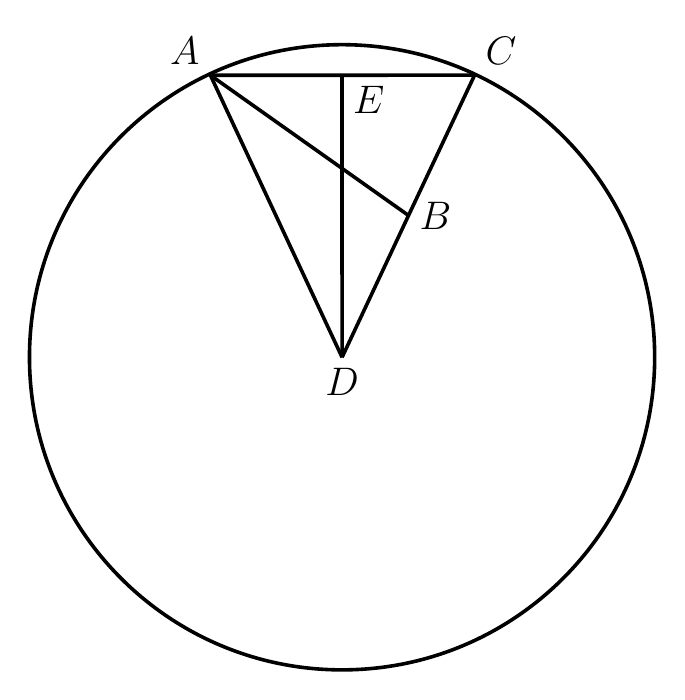
\begin{tikzpicture}[line width=1.3pt, line join=round]
\coordinate (A) at (-1.681,3.612);
\coordinate (B) at (0.835,1.831);
\coordinate (C) at (1.674,3.613);
\coordinate (D) at (-0.009,0.030);
\coordinate (E) at (-0.010,3.612);



\draw (D) circle (3.970);


\draw (A) -- (E) -- (C);
\draw (E) -- (D);


\draw (A) -- (D);
\draw (C) -- (B) -- (D);
\draw (A) -- (B);


\node[above left] at (A) {\fontsize{13.5}{16.2}\selectfont $A$};
\node[above right] at (C) {\fontsize{13.5}{16.2}\selectfont $C$};
\node[below right] at (E) {\fontsize{13.5}{16.2}\selectfont $E$};
\node[below] at (D) {\fontsize{13.5}{16.2}\selectfont $D$};
\node[right] at (B) {\fontsize{13.5}{16.2}\selectfont $B$};
\end{tikzpicture}
\end{document}